\documentclass[../root]{subfiles}
\graphicspath{{_images/}{../_images/}}

\begin{document}

    \chapter{Effects of parental leave policies on female career and fertility choices}

    \begin{shortsummary}
        \begin{itemize}
            \item \authoryear{Yamaguchi2019}
            \item \RQ{Does an expansion of the parental leave (PL) policies lead to a higher fertiliy and labor force participation rate of mothers of young children?}
            \item \answer{A dynamic discrete choice structual model of female employment and fertility decisions that incorporates job protection and cash benefits of PL legislation}
            \item \result{Introducing an initial 1-year job protection policy increases maternal employment significantly, but extending the existing job protection period from 1 to 3 years has little effect.}
        \end{itemize}
    \end{shortsummary}

    \section{Introduction}

    \paragraph{This paper explores the effect of the parental leave legislation.}

    \begin{itemize}
      \item Parental leave, or \textbf{PL}, is mandated in most developed countries, but the generocity of PL legislation varies significantly across countries (Figure 1).
      \begin{itemize}
        \item The duration of \textbf{job-protected leave} (育児休暇).
        \item The replacement rate of \textbf{cash benefits} (出産・児童手当).
      \end{itemize}
      \item Policy makers are interested in expanding their PL policies to rersolve the conflict between work and family life.
      \begin{itemize}
        \item Possible way to predict likely outcomes before a policy reform:
        \begin{itemize}
          \item to learn from the experiences of countries where the most generous PL policies are already mandated: not fully generalized
          \item to conduct a small-scale social experiment: costly and politically infeasible.
        \end{itemize}
      \end{itemize}
      \item To approach to ex ante policy evaluation, this paper constructs a \textbf{structual dynamic discrete choice model} of women's employment and fertility.
    \end{itemize}

    \begin{figure}
      \centering
      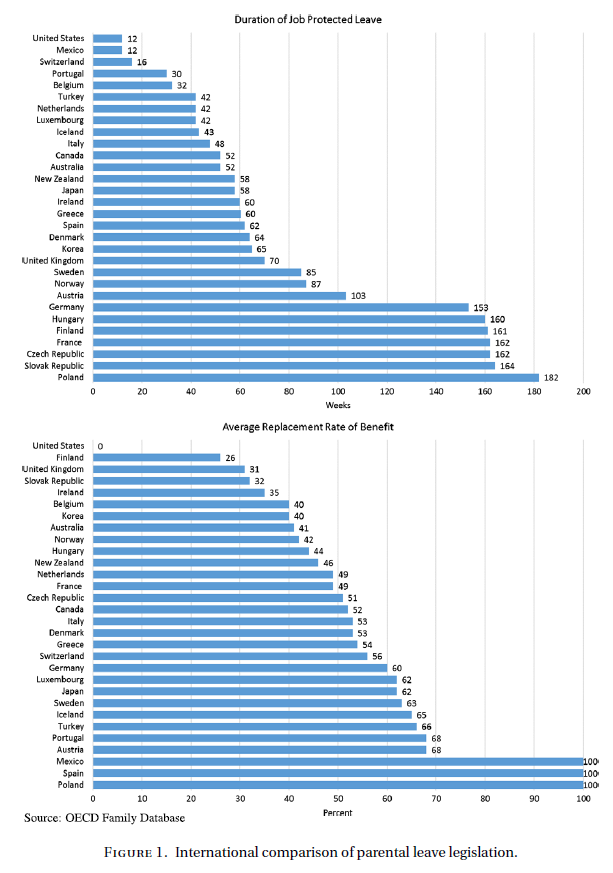
\includegraphics[scale = 1.3]{0619tanji/F1}
      \label{F1}
    \end{figure}

    \paragraph{Dynamic discrete choice model}

    \begin{itemize}
      \item A model of women’s employment and fertility that incorporates job protection and cash benefits of PL
      \begin{itemize}
        \item In each period, a woman decides on her employment sector, PL takeup, and conception.
        \item When a mother of a young child works, she not only pays child care costs, but also derives negative nonpecuniary utility of work because she values the time with her young child.
        \item Also incorporate the entry cost to employment for women.
      \end{itemize}
      \item Related papers
      \begin{itemize}
        \item Eckstein and Wolpin (1989), van der Klaauw (1996), Altug and Miller (1998), Francesconi (2002), Sheran (2007), Keane and Wolpin (2007, 2010), Adda, Dustmann, and Stevens (2017), and Gayle andMiller (2012).
      \end{itemize}
    \end{itemize}

    \paragraph{Summary of Results}

    \begin{itemize}
      \item The counterfactual simulations
      \begin{itemize}
        \item 1-year job protection increases maternal employment after childbearing with effects that last for several years, compared with no mandated PL.
        \begin{itemize}
          \item Job protection allows women to suspend working prior to childbirth without losing their jobs: no entry costs to return to work.
        \end{itemize}
        \item Extending the duration of job protection from 1 to 3 years has little effect.
        \begin{itemize}
          \item Nonpecuniary utility of work is very negative when the child is newborn but becomes much smaller as the child grows to age 1 year or older.
        \end{itemize}
        \item Policy effects on fertility seem modest for both 1- and 3-year job protection.
        \item Raising the rate of cash benefits that accrue with job-protected PL has modest effects on maternal work and fertility.
        \begin{itemize}
          \item Overall, neither the duration of job protection nor cash benefits in the current PL legislation create a binding constraint for mothers of young children.
        \end{itemize}
      \end{itemize}
    \end{itemize}


    \paragraph{Contribution}

    \begin{itemize}
      \item To use a structural estimation approach to evaluate potential PL reforms.

      Previous approach:
      \begin{itemize}
        \item difference-in-differences (DID) estimator (Ruhm (1998), Baum (2003a), and Baker andMilligan (2008a))
        \item regression discontinuity designs (Lalive and Zweimu\"{u}ller (2009), Sch\"{o}nberg and Ludsteck (2014), and Lalive, Schlosser, Steinhauer, and Zweim\"{u}ller (2014))
      \end{itemize}
      \item The structural model helps one understand how PL policies affect maternal work and speculate about the potential policy effects in a given country.
    \end{itemize}
    \begin{itemize}
      \item Technical: Combining following three methods:
      \begin{enumerate}
        \item Kasahara and Shimotsu (2011): allows for permanent unobserved heterogeneity.
        \item Arcidiacono and Jones (2003): Expecation-Maximization algorithm
        \item Aecidiacono, Beyer, Bugni, and James (2013): approximation method for the value function.
      \end{enumerate}
    \end{itemize}


    \section{Institutional Background}

    \paragraph{The employment sector in Japan}

    \begin{itemize}
      \item Regular employment: under a permanent contract and a full-time job
      \item Nonregular employment: under a limited-termcontract and a part-time job.
    \end{itemize}

    Regular jobs are usually superior to nonregular jobs in terms of hourly wages, nonwage benefits, employer-sponsored training, and eligibility for mandated PL (see Kambayashi and Kato (2013)).

    \begin{figure}[h]
      \centering
      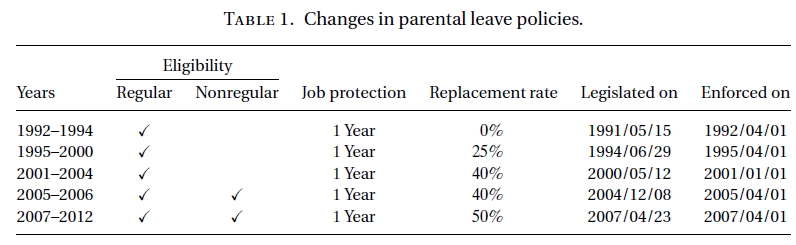
\includegraphics[scale = 1]{0619tanji/T1}
      \label{T1}
    \end{figure}

    \paragraph{History of PL}

    \begin{itemize}
      \item PL in Japan was first enforced in 1992.
      \begin{itemize}
        \item Until 2005 it was eligible for only regular workers.
      \end{itemize}
      \item Cash benefits were first introduced in 1995.
      \begin{itemize}
        \item Cash benefits are not financed directly by employers, but rather by employment insurance (same as Austria, Canada, and Germany).
        \item An important difference from some other countries is that cash benefits are tied to the job from which PL is taken.

        $\Rightarrow$ PL takers are expected to return to the pre-leave job.
        \begin{itemize}
          \item PL takers must apply through employers to receive cash benefits
          \item Although there is no legal penalty for not returning, about 90\% of PL takers are employed 1 year after childbearing
        \end{itemize}
      \end{itemize}
      \item Notes
      \begin{itemize}
        \item If a PL taker gives birth during her leave, she can renew the PL and receive cash benefits.
        \item Very few fathers take PL. In 2010, the PL takeup rate among fathers was 1.38\%, and more than half of male PL takers were on leave for only 1 week.
      \end{itemize}
    \end{itemize}

    \section{Data}
    \subsection{Overview of the data structure}

    \paragraph{Japanese Panel Survey of Consumers (JPSC)}

    by The Institute for Research onHousehold Economics.

    \begin{itemize}
      \item A panel survey of a representative sample of women aged 24-52
      \item started in 1993, with 1,500 women aged 24-34
      \item asks about: every year
      \begin{itemize}
        \item marriage, fertility
        \item their and their spouse's work.
      \end{itemize}
      \item As of 2008, the JPSC had sampled 2,284 women.
      \item Observation period: 1993 - 2011
    \end{itemize}

    \paragraph{Data processing}

    \begin{itemize}
      \item A sample of married women who completed schooling and were not employed.
      \item Observation with missing values except for self-earnings are omitted.
      \item $N = 14,907$ person $\times$ year.
    \end{itemize}

    \begin{figure}[h]
      \centering
      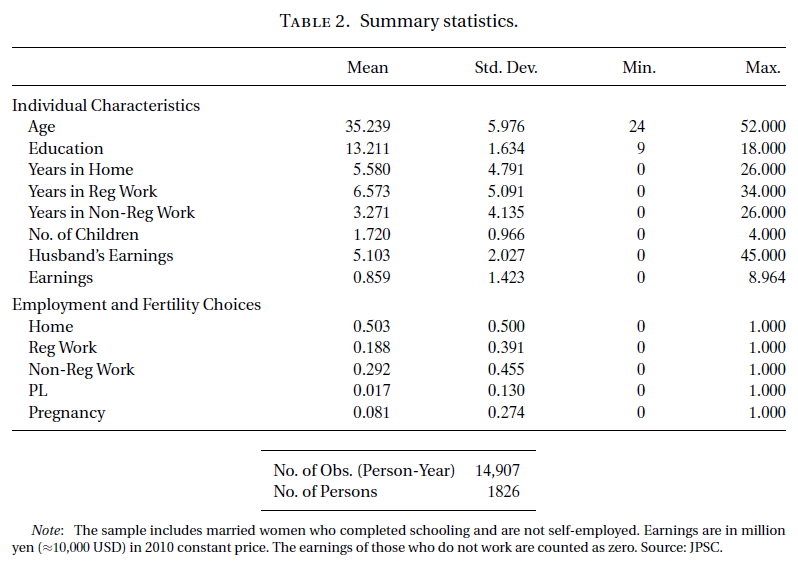
\includegraphics[scale = 1]{0619tanji/T2}
      \label{T2}
    \end{figure}

    \begin{itemize}
      \item The age of sampled individuals ranges from 24–52 years, covering more than 89\% of childbirths.
    \end{itemize}


    \subsection{Descriptive analysis}

    \paragraph{Life-cycle profiles}

    \begin{itemize}
      \item Women gradually return to the labor market after childbearing, but largely to nonregular employment.
      \begin{itemize}
        \item The percentage staying at home at age 30 years is high, at 59\% , but this gradually decreases with age. (comparable with those from the Labor Force Survey 2010)
      \end{itemize}
      \item The percentage of PL takers is small, at 3.7\% at age 30 years, and gradually decreases with age.
      \item Self and husbands earnings increase over time.
    \end{itemize}

    \begin{figure}[h]
      \centering
      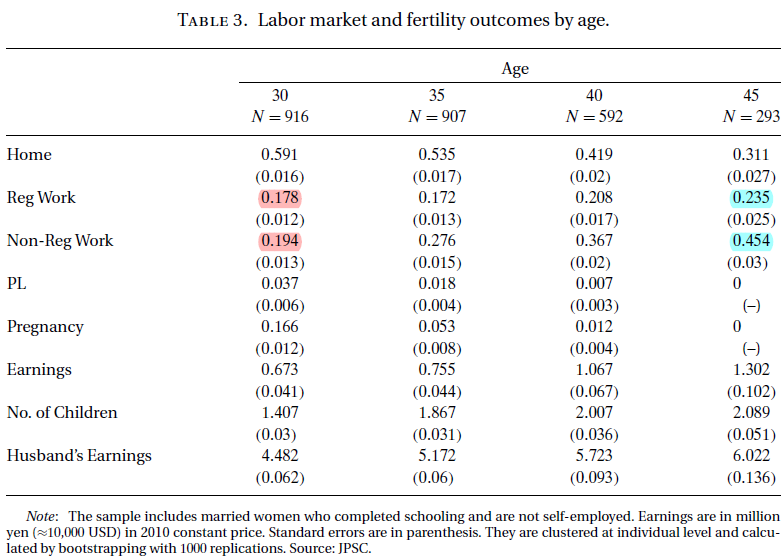
\includegraphics[scale = 1]{0619tanji/T3}
      \label{T2}
    \end{figure}

    \paragraph{Employment transition}

    \begin{itemize}
      \item The vast majority of PL takers in $t − 1$ return to work in $t$.
      \item Employment choices are serially correlated except for PL.
      Possible sources:
      \begin{itemize}
        \item heterogeneity
        \begin{itemize}
          \item sector-specific human capital
          \item an entry barrier to employment sectors
        \end{itemize}
        \item state dependence
      \end{itemize}
    \end{itemize}


    \begin{figure}[h]
      \centering
      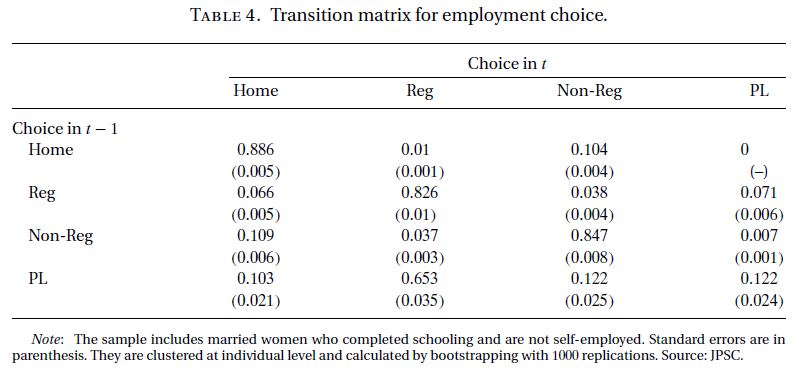
\includegraphics[scale = 1]{0619tanji/T4}
      \label{T2}
    \end{figure}

    \paragraph{PL take-up rate}

    \begin{itemize}
      \item Among women who give birth, only about 30\% hold a job eligible for PL at childbirth.
      \item Although there is no penalty for not returning, about 90\% of leave takers return to employment a year after childbearing
      \begin{itemize}
        \item about 30\% actually end up quitting their jobs without collecting cash benefit
      \end{itemize}
    \end{itemize}

    \begin{figure}[h]
      \centering
      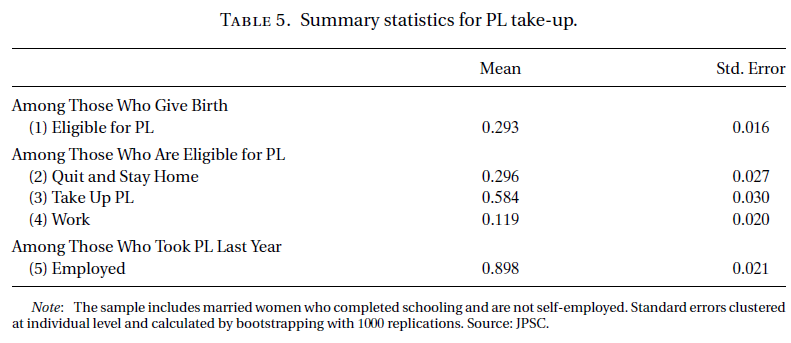
\includegraphics[scale = 1]{0619tanji/T5}
      \label{T2}
    \end{figure}


    \section{Model}

    \subsection{Setup}

    \paragraph{A dynamic discrete choice framework}

    \begin{itemize}
      \item In each calendar year $t$, a forward-looking woman maximizes her present value of lifetime utility by deciding on labor supply and fertility.
      \item She retires from the labor market and receives the terminal value of zero at age 65 years.
      \item Individuals differ in their unobserved characteristics, including
      \begin{itemize}
        \item permanent skills in regular and nonregular sectors
        \item nonpecuniary utility from work and children
        \item their husbands’ permanent skills.
      \end{itemize}
    \end{itemize}

    \paragraph{Choices}

    \begin{itemize}
      \item A vector of decision variables is
      \[
      d_{it} = (d_{h, it}, d_{r, it}, d_{n, it}, d_{l, it}, d_{f, it})
      \]
      Each binary variable indicates for individual $i$ in period $t$
      \begin{itemize}
        \item staying at home
        \item working in the regular employment sector
        \item working in the nonregular employment sector
        \item taking PL

        The labor supply choices are exhaustive and mutually exclusive.

        and
        \item whether to conceive or not
      \end{itemize}
      \item Taking PL is in the choice set only when an individual has been employed in the previous year in either the regular or nonregular sector and has a child aged between 0 and 2

      (many women in the data who have been employed in the noncovered sector and/or have a child aged 1 year or older report their PL take-up.)
      \item A woman does not make a fertility decision after age 45 years.
    \end{itemize}

    \paragraph{State Variables}

    \begin{itemize}
      \item A vector of her state variables: $S_{it}$:
      \begin{itemize}
        \item sectore-specific experiences: $(x_{h, it}, x_{r, it}, x_{n, it})$
        \item age: $a_{it} = $ her own, $a_{k, it} = $ her youngest child
        \item \# of children: $n_{it}$
        \item earnings of the male spouse $y_{m, it}$
        \item lagged choices $d_{it-1}$
        \item lagged employment status $e_{it - 1} = (e_{r, it-1}, e_{n_it-1})$, where $e_{r, it-1} + e_{n_it-1} \leq 1$.
        \item calendar year $t$.
      \end{itemize}
      \item The transition of state variables is deterministic except for the earnings of the male spouse.
      \item Individuals expect that the calendar year as a state variable does not change from this year to next, which also implies that individuals expect the unemployment rate to remain at the current level.
    \end{itemize}

    \subsection{Preference}

    \paragraph{Consumption}

    \begin{align*}
      u(C_{it}, n_{it}, d_{it}) &= \alpha (d_{it}, n_{it}) \cdot C_{it} \\
      &= [\alpha_1 + \alpha_2 d_{r, it} + \alpha_3 d_{n, it} + \alpha_4 \sqrt{n_{it}}] \cdot C_{it}
    \end{align*}

    \begin{itemize}
      \item Nonseparability of consumption and nonmarket time specification: Eckstein and Wolpin (1989).
      \begin{itemize}
        \item $\alpha_2 < 0, \alpha_3 < 0$: women having higher-income husbands are less likely to work, which is widely observed across countries
      \end{itemize}
    \end{itemize}

    where
    \[
    C_{it} = y_{m, it} + d_{r, it} y_{n, it} + d_{l, it} b_{it} - (d_{r, it} + d_{n, it}) CC(a_{k, it})
    \]

    \begin{itemize}
      \item $y_{m, it}$, $y_{n, it}$: earnings of her husband and herself, respectively.
      \item $b_{it}$ is the cash benefit for PL
      \item $CC(\cdot)$: the child care cost
    \end{itemize}

    \paragraph{Nonpecuniary utility from labor supply choices}

    \begin{itemize}
      \item Individuals derive nonpecuniary utility from work, normalized by setting the utility of staying at home zero and parametrized as follows:
      \begin{align*}
        v_{j, it} = & \gamma_{ij, 1} + \gamma_{j, 2} d_{h, it-1} + \gamma_{j, 3} e_{k \neq j, it - 1} + \gamma_{j, 4} d_{l, it - 1} e_{j, it-1} \\
        &+ \gamma_{j, 5} \sqrt{n_{it}} + \gamma_{j, 6}(\alpha_{k, it}) + \gamma_{j, 7} \text{UR}_t
      \end{align*}
      \begin{itemize}
        \item Regular and nonregular works are distingished in $j = r, n$.
        \item The second, third, and fourth terms are the entry costs to the employment sector $j$ from each state.
        \begin{itemize}
          \item $\gamma_{j, 4}$ is expected to be close to zero: job protection helps women return to work after childbearing, and this is particularly useful in countries where the labor market is rigid, such as Japan and Southern European countries.
        \end{itemize}
      \end{itemize}
    \end{itemize}


    \paragraph{Taking parental leave}

    \begin{itemize}
      \item The nonpecuniary utility for PL take-up is:
      \[
      v_{l, it} = v_{il, 1} + v_{l, 2} e_{r, it-1} + v_{l, 3} \text{ELG}_{it} + v_{l, 4} d_{l, it-1} (1 - \text{ELG}_{it})
      \]
      \begin{itemize}
        \item $\text{ELG}_{it}$: a dummy that takes 1 if individual $i$ is legally entitled to PL in year $t$.
        \item This paper assumes that not all eligible women take PL (see Table 5).
        \begin{itemize}
          \item About 30\% of eligible women quit their jobs without collecting cash benefits.
          \item To rationalize this observed PL take-up behavior, this paper assumes the existence of nonpecuniary cost of taking up PL.
        \end{itemize}
      \end{itemize}
    \end{itemize}

    \paragraph{Nonpecuniary utility from children}

    \begin{itemize}
      \item At the time of conception, a married woman derives utility from children as a lump sum,
      \[
      v_{f, it} = \gamma_{if, 1} + \gamma_{f, 2} d_{r, it} + \gamma_{f, 3} d_{n, it} + \gamma_{f, 4} (a_{it}) + \gamma_{f, 5}(a_{k, it}, n_{it})
      \]
    \end{itemize}



    \subsection{Income and cost of child care}

    How to specify $y_{m, it}$, $y_{n, it}$

    \paragraph{Self-earnings}

    \[
    y_{j, it} = \omega_{j1, 1} + \omega_{j, 2} (x_{j, it}, x_{k \neq j, it}) + \omega_{j, 3} + \omega_{j, 4} (d_{it-1}) + \omega_{j, 5}\text{UR}_t + \eta_{j, it}
    \]

    $j = n, r$

    \begin{itemize}
      \item Intercept accounts for heterogeneous sector-specific skills.
      \item The second term: experiences in each sectors.
      \item The third term:  years spent at home, or permanent human capital depreciation.
      \item The fourth term: adjustment cost to a new work environment.
      \item $\text{UR}$ unemployment rate.
    \end{itemize}

    \paragraph{Cash benefits}

    \[
    b_{it} = R_t \min \left[ 5.112, d_{r, it - 1} \dfrac{12}{15}\hat{y}_{r, it} + d_{n, it-1} \dfrac{12}{13} \hat{y}_{n, it} \right]
    \]

    \begin{itemize}
      \item $R_t$: replacement rate.
      \item $\hat{y}_{j, it}$: the predicted earnings
      \item Benefits are replaced up to 5.112 milloion JPY per year.
      \item In the JPSC, gross labor earnings includeing bonus are reported: $\dfrac{12}{15}$ and $\dfrac{12}{13}$ are multiplied to adjust this possible downward scale.
    \end{itemize}

    \paragraph{Earnings of husband}

    \begin{align*}
      y_{m, it} = &\omega_{mi, 1} + \omega_{m, 2} y_{m, it-1} + \omega_{m, 3} + \omega_{m, 4} (a_{k, it}, n_{it}) + \omega_{m, 5} (d_{it}) \\
      & + \omega_{m, 6} + \eta_{m, it}
    \end{align*}

    \paragraph{Cost for child care}

    \begin{align*}
      CC(a_{k, it}) = & [I(a_{k, it} = 0) \cdot 43,739 + I(a_{k, it} = 1) \cdot 40,660 \\
      &+ I(a_{k, it} = 2) \cdot 38,179 + I(3 \leq a_{k, it} \leq 5) \cdot 34,181] \times 12/1,000,000
    \end{align*}

    \begin{itemize}
      \item Reported child care cost raises the concern of endogeneity biases.
      \item This paper uses the average of the list prices.
    \end{itemize}


    \subsection{Utility Maximization}

    \begin{itemize}
      \item The objective of a married woman is to maximize
      \begin{align*}
        V(S_{it}, \epsilon_{it}) = & \max_{d_{it}} u(C_{it}, n_{it}, d_{it}) + d_{r, it} v_{r, it} + d_{n, it} v_{n, it} + d_{l, it} v_{l, it} + d_{f, it} v_{f, it} + \epsilon_{it}(d_{it}) \\
        &+ \beta E[V(S_{it+1}, \epsilon_{it+1}) | S_{it}, d_{it}]
      \end{align*}
      \begin{itemize}
        \item $\beta$: discount factor
        \item $\epsilon_{it}(d_{it})$ unobservable choice-specific shock, which follows a generalized extreme value distribution.
        \item The choice probability is modeled by the generalized nested logit model that allows for overlapping nests (Wen and Koppelman, 2001)
      \end{itemize}
    \end{itemize}

    \subsection{Unobserved Heterogeneity}

    Permanent unobserved heterogeneity is modeled as a finite mixture.

    \begin{itemize}
      \item Individuals are one of the $K$ types, but the type of an individual is not observed.
      \item The probability of being type $k$ to depend on the observed characteristics and choices in year $t = \tau(i)$: the first year when individual $i$ is observed in the data (cf. Wooldridge, 2005)
      \item Define a vector $z$ in year $\tau(i): z_{i \tau (i)} = (d_{i}, S_{i \tau (i)}, \text{edu}_i)$.
    \end{itemize}

    Then the probability that individual $i$ is type $k$ is given by
    \[
    p_{k}(z_{i \tau (i)}) = \dfrac{\exp (\pi_k' z_{i \tau (i)})}{\sum_{\kappa = 1}^K \exp (\pi_k' z_{i \tau (i)})}
    \]
    The parameters for the first type is set to zero so that $\pi_{\kappa = 1} = 0$


    \subsection{Comparison with previous structual models}

    \begin{itemize}
      \item Literature
      \begin{itemize}
        \item Gayle and Miller (2012): the role of job protection or PL take-up is not considered.
        \item Adda, Dustmann, and Stevens (2017): assume that all women giving birth take PL and receive job protection and cash benefits.
      \end{itemize}
      $\Rightarrow$ Not modeling PL take-up and instead assuming that all women take PL may result in biased estimates for the effects of PL policies.
      \item The closest paper: Lalive et al. (2014): based on the continuous-time job search model of Frijters and van der Klaauw (2006).

      The important differnce of the paper is:
      \begin{itemize}
        \item Modeling PL take-up
        \item Allowing for fertility choice
        \item Considering occupational choices (regular vs. nonregular jobs)
      \end{itemize}
    \end{itemize}

    \section{Estimation Strategy}

    \subsection{Estimation algorithm}

    The model is estimated by the maximum likelihood method.

    \begin{itemize}
      \item The maximum is found by combining the three algorithms that accelerate computation.
      \begin{enumerate}
        \item Kasahara and Shimotsu (2011)
        \item Arcidiacono et al. (2013)
        \item Arcidiacono and Jones (2003)
      \end{enumerate}
      \item If interested, please check online Appendix B.
    \end{itemize}

    \subsection{Identification}

    \begin{itemize}
      \item Difference between DID: Using policy reform in PL, we may estimate the effect of job protection and the cash benefits.
      \begin{itemize}
        \item In structural estimation, selection into sectors is modeled to avoid this bias.
        \begin{itemize}
          \item Policy reform in in the eligibility condition and the replacement rate.
          \item Workers who entered under job protection are nonregular workers.
        \end{itemize}
        \item Small sample size.
        \begin{itemize}
          \item The employment rate prior to childbirth is low, the sample size for the DID approach is small.
          \item In structural estimation, we can check the internal validity of the esitmation.
          \item (misspecification of the structural model is a legitimate concern)
        \end{itemize}
      \end{itemize}
    \end{itemize}

    \section{Estimation Results}
    \subsection{Parameter estimates}

    \paragraph{Marginal utility of consumption}

    \begin{itemize}
      \item The estimated marginal utility of consumption is positive, but decreases when women work either in regular or nonregular sectors.
      \item A wife’s labor force participation decreases with her husband’s earnings, all else being equal.
    \end{itemize}

    \begin{figure}[h]
      \centering
      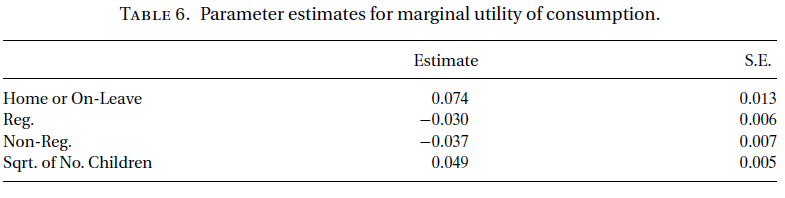
\includegraphics[scale = 1]{0619tanji/T6}
      \label{T5}
    \end{figure}

    \paragraph{Nonpecuniary utility of work}

    \begin{figure}[h]
      \centering
      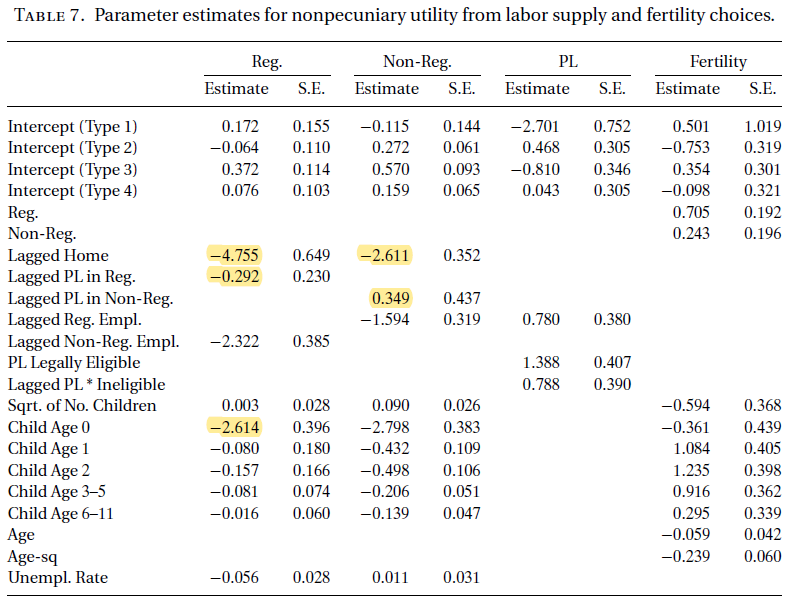
\includegraphics[scale = 1]{0619tanji/T7}
      \label{T6}
    \end{figure}

    \begin{itemize}
      \item The entry costs to employment sectors from home are large: job protection is expected to help mothers of young children return to the labor market quickly.
      \item Having a young child decreases the nonpecuniary utility of work in both sectors, and the negative effect is particularly large when the child is less than 1 year of age.
      \begin{itemize}
        \item On the other hand, PL may not be as valuable for mothers of children aged 1 year or older because the negative effect on the nonpecuniary utility quickly fades after the child’s first birthday.
      \end{itemize}
    \end{itemize}

    \paragraph{Transaction cost of PL take-up}

    \begin{itemize}
      \item The nonpecuniary utility of PL take-up varies greatly by unobserved type: PL is generally unpleasant for type 1 women, but it is less so for other types: the financial incentives of PL are likely to be irrelevant for type 1 (row 1-4).
      \item Legal eligibility for PL reduces the transaction cost of PL take-up (row 12, 13)
      \item The transaction cost of PL take-up is also found to be lower in the regular sector (row 10).
    \end{itemize}

    \paragraph{Utility from children}

    \begin{itemize}
      \item Utility decreases with the number of existing children and when the mother has a child aged less than 1 year.
    \end{itemize}

    \paragraph{Correlation structure of error terms}

    \begin{itemize}
      \item The dissimilarity parameters measure the degree of independence among alternatives within the nest and take a value between zero and one. \item The estimates are smaller than one, implying that choices are correlated within each nest.
      \item
    \end{itemize}

    \paragraph{Earnings functions}

    \begin{itemize}
      \item Experience in an individual’s own sector increases earnings.
      \item Years at home reduce earnings in both sectors, which implies earnings capacity depreciates while at home or on leave.
      \item A temporary earnings penalty was also observed for those who stayed at home or had been on leave in the last year.
    \end{itemize}

    \subsection{Model fit}

    \begin{itemize}
      \item 30 simulations using the model from the initial observations for each individual in the data until the period ending with the last appearance.
      \item The model in this paper highly fits the data:labor market outcomes, transition matrix and PL take-up rate.
      \item Also fits the policy reform: the expansion of job protection to nonregular workers in 2005
    \end{itemize}

    \begin{figure}[h]
      \centering
      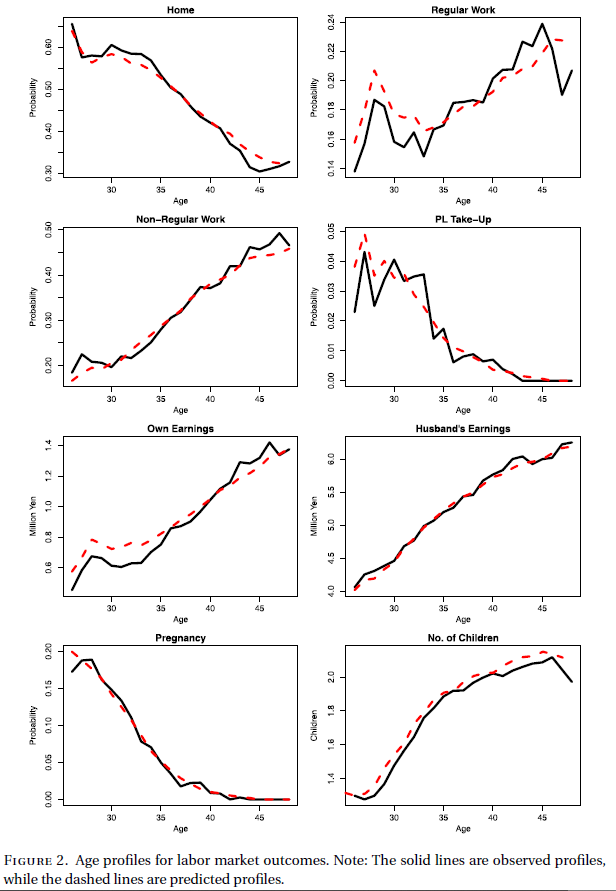
\includegraphics[scale = 1]{0619tanji/F2}
      \label{F2}
    \end{figure}

    \begin{figure}[h]
      \centering
      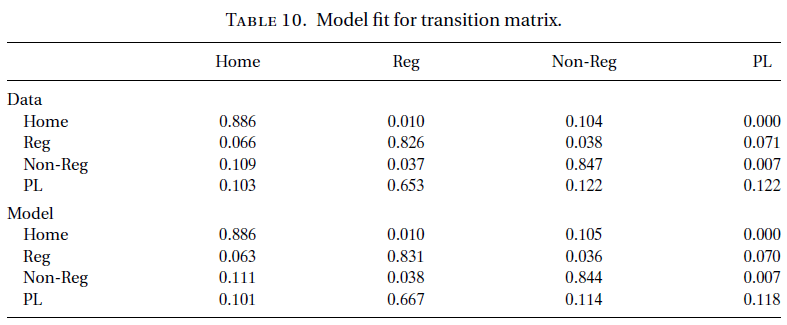
\includegraphics[scale = 1]{0619tanji/T10}
      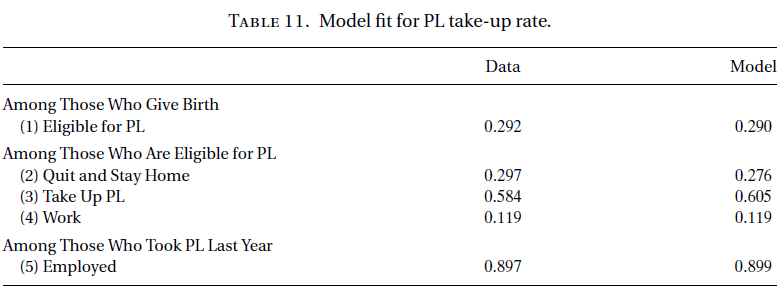
\includegraphics[scale = 1]{0619tanji/T11}
      \label{T1011}
    \end{figure}

    \subsection{Discussion}

    \begin{itemize}
      \item Two important assumption
      \begin{itemize}
        \item Omitting saving decisions
        \item Taking husband's labor supply and earnings as exogenous
      \end{itemize}
      \item Regression: Do assets have an additional explanatory power for labor supply and fertility choices?
      \begin{itemize}
        \item Assets add very little to explanation of the probabilities of choosing to stay at home
        \item However, assets are significantly correlated with the PL take-up rate, the p-value being .001.
      \end{itemize}
      \item Comparison between before/after the PL policy change in 2005
      \begin{itemize}
        \item Average weekly hours of work decreased slightly from 51845 to 51175, while average annual earnings increased slightly from 5112 to 5328.
        \item Effect on husbands in response to the PL reform are modest compared with large changes in mothers’ PL take-up and non-regular employment rates.
      \end{itemize}
    \end{itemize}

    \begin{figure}[h]
      \centering
      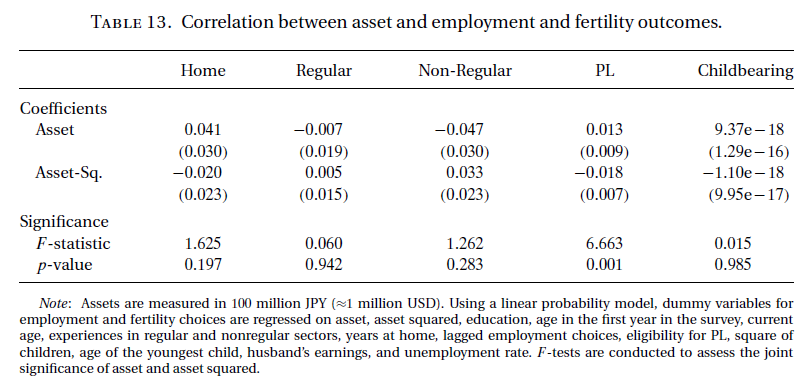
\includegraphics[scale = 1]{0619tanji/T13}
      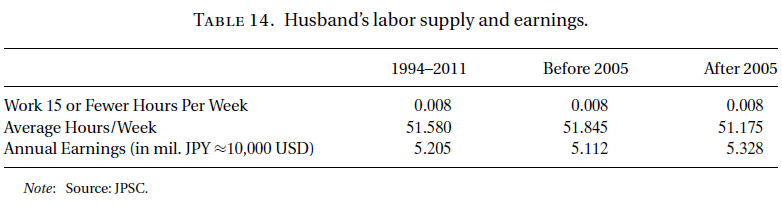
\includegraphics[scale = 1]{0619tanji/T14}
      \label{T13}
    \end{figure}

    \section{Counterfactual Simulations}

    Using the estimated model, This paper simulates labor supply and fertility decisions of women under different policy scenarios. Each individual is simulated 1000 times.

    \subsection{Job protection}

    Three simulations:
    \begin{enumerate}
      \item no PL
      \item 1-year job protection
      \item 3-year job protection
    \end{enumerate}
    In all scenarios, no cash benefits are paid.

    \paragraph{The probability of work}

    \begin{itemize}
      \item The probability of work in the childbearing year drops to .19 without mandated PL.
      \item The probability of work 1 year after childbearing is .33 without mandated PL, while 1- and 3-year job protection, this increases to .54.
    \end{itemize}
    These policy effects on maternal work persist as long as 10 years after childbearing, but expanding job protection from 1 to 3 years has little marginal effect.

    \paragraph{PL take-up rates}

    \begin{itemize}
      \item One- and 3-year job protection boost take-up rates by more than four times as where PL is not mandated (.12).
      \item The take-up rates a year after childbearing drop substantially, even if 3-year job protection is approved.
    \end{itemize}

    \paragraph{Additional remarks}

    \begin{itemize}
      \item Percentage of mothers working in the regular sector
      \begin{itemize}
        \item Job protection increases the percentage of mothers working in the regular sector, while it decreases the proportion of mothers working in the nonregular sector.
        \item The policy effects persist 10 years after childbirth.
      \end{itemize}
      \item Job protection appears to have a small positive effect on fertility.
    \end{itemize}


    \begin{figure}[h]
      \centering
      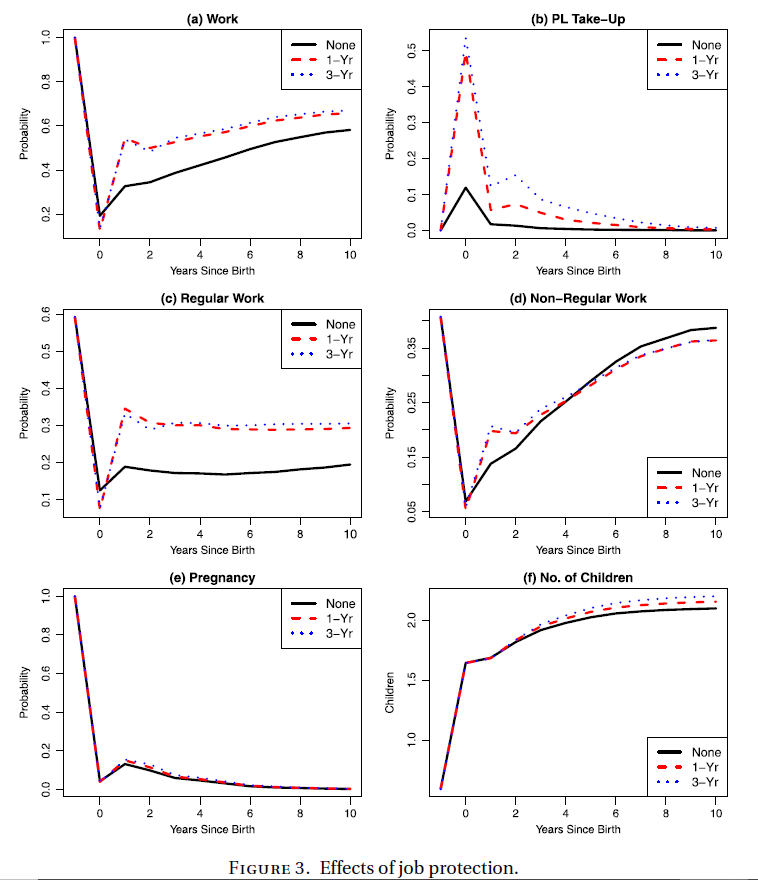
\includegraphics[scale = 1]{0619tanji/F3}
      \label{F3}
    \end{figure}

    \paragraph{Policy effects on accumulated income, consumption, and welfare}

    \begin{figure}[h]
      \centering
      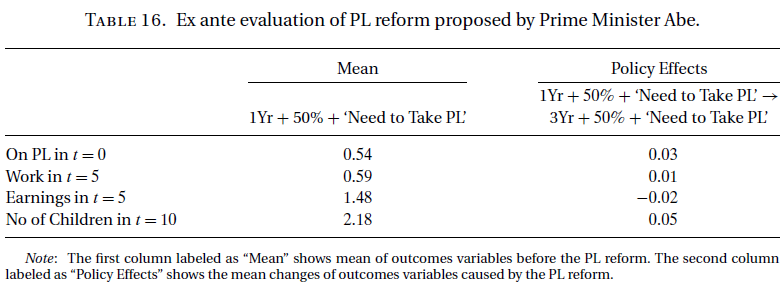
\includegraphics[scale = 1]{0619tanji/T16}
      \label{T16}
    \end{figure}

    \begin{itemize}
      \item The introduction of 1-year job protection increases accumulated income from 10.56 to 14.81 or by 40\%
      \item It also increases accumulated consumption from 74.39 to 77.77.
    \end{itemize}


    \subsection{Cash benefits}

    Three senarios where 1-year job protection.

    \begin{enumerate}
      \item no cash benefits are paid
      \item mothers can receive cash benefits even if they do not apply for job-protected PL.
      \item mothers must apply for job-protected PL to receive cash benefits  *Japanese PL system.
    \end{enumerate}

    The replacement rate is set at 50\%.

    \begin{figure}[h]
      \centering
      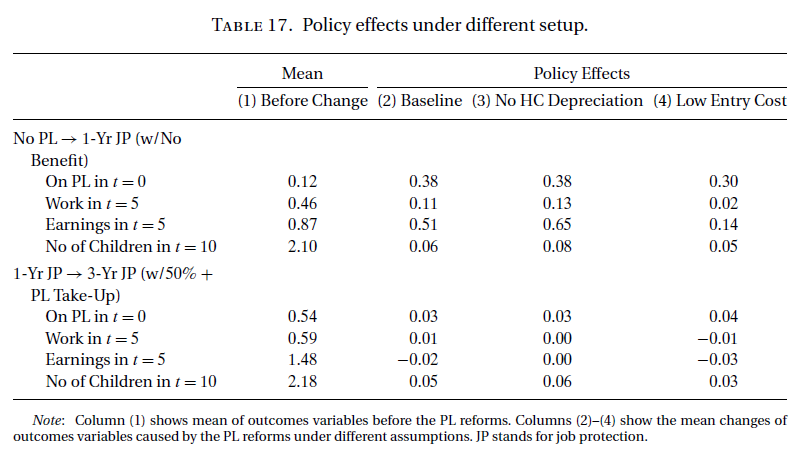
\includegraphics[scale = 1]{0619tanji/T17}
      \label{T17}
    \end{figure}

    \begin{itemize}
      \item The effects on the PL take-up rate are modest.
      \begin{itemize}
        \item When the replacement rate increases from 0\% to 50\%, the take-up rate increases by two percentage points.
        \item The effects on probability of work, earnings, and fertility are also modest, although positive.
      \end{itemize}
      \item Welfare effects
      \begin{itemize}
        \item Tying cash benefits to job protected PL increases income and consumption but decreases welfare for lost time at home.
      \end{itemize}
    \end{itemize}



    \subsection{Other family-friendly policies}

    \begin{itemize}
      \item Baby bonuses
      \begin{itemize}
        \item Baby bonuses increase the fertility rate and that policy effects increase with the size of the bonus.
        \item However, it also decreases the mother’s labor supply and earnings.
      \end{itemize}
      \item Child care subsidy
      \begin{itemize}
        \item Child care subsidies modestly increased both fertility and mother’s labor supply.
      \end{itemize}
    \end{itemize}

    PL legislation generally has few fertility effects. There is a fundamental trade-off between a woman’s career and children, and that promoting both at the same time is quite challenging for policy makers.

    Assessing the effects of a child care subsidy in the Japanese context is not straightforward in the current model for two reasons.

    \begin{itemize}
      \item the model does not allow for the use of free or cheap informal child care arrangements provided by grandparents.
      \item Excess demand for childcare in Japan.
    \end{itemize}

    \begin{figure}[h]
      \centering
      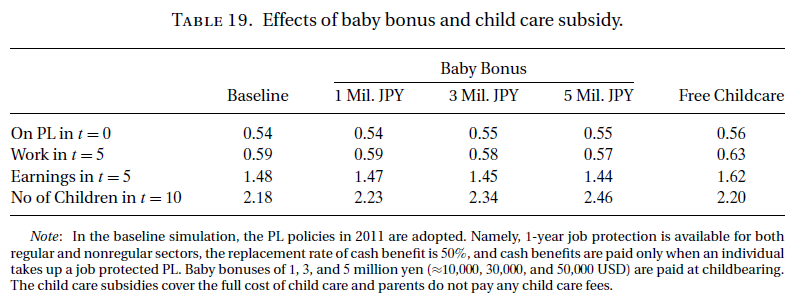
\includegraphics[scale = 1]{0619tanji/T19}
      \label{T10}
    \end{figure}

    \section{Concluding Remarks}

    \begin{itemize}
      \item The model and estimation method offer a useful tool to predict the potential effects of parental leave in other countries such as the US.
      \item One area to examine in future work is the interaction with other pro-family policies intended to support working mothers, such as child care expansion.
    \end{itemize}

    \biblio

\end{document}
